\begin{frame}{Αισθητήρας lidar δισδιάστατων μετρήσεων απόστασης}

  \noindent\makebox[\linewidth][c]{%
  \begin{minipage}{\linewidth}
    \begin{minipage}{0.3\linewidth}
      \begin{figure}
        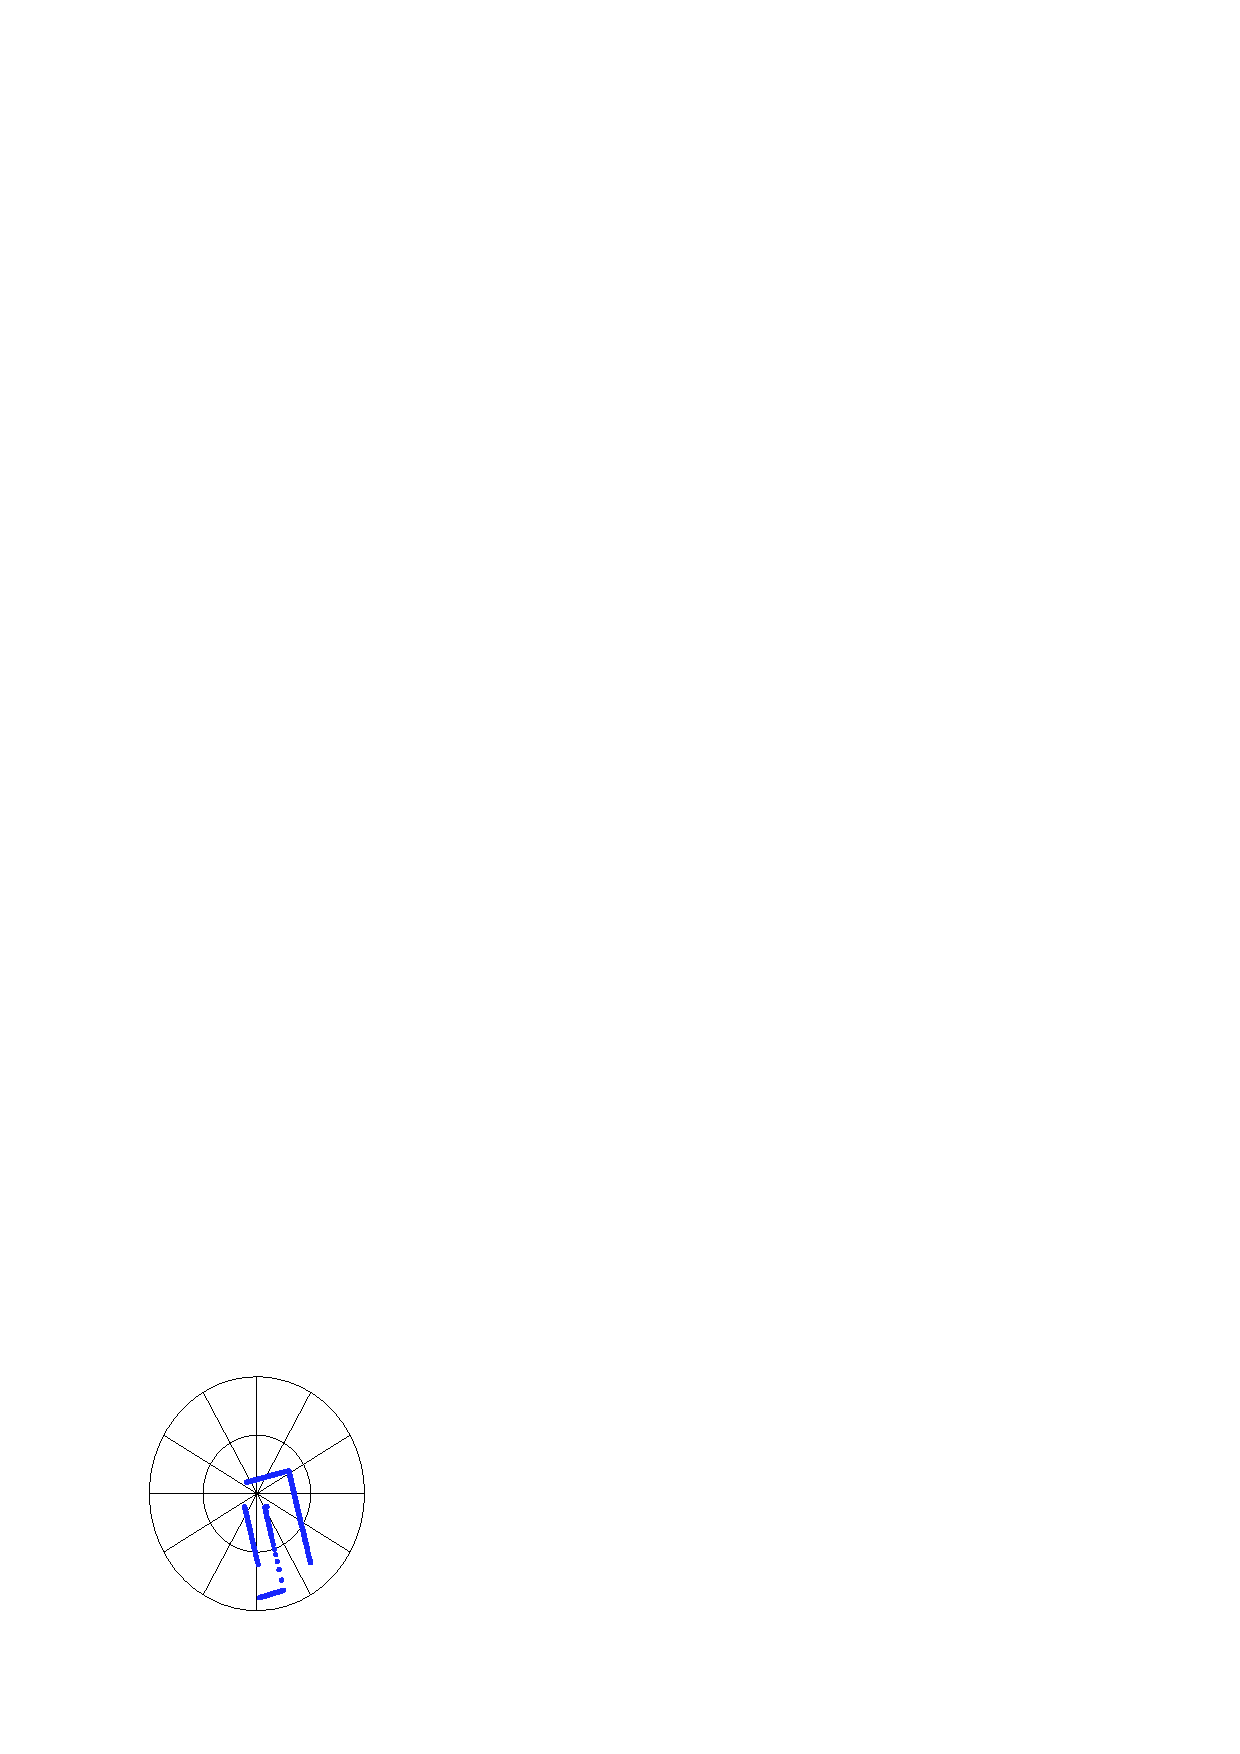
\includegraphics[scale=0.1]{./figures/slides/ch4/gazebo_scan_np.png}
        \caption{\scriptsize Κάτοψη περιβάλλοντος και ακτίνες αισθητήρα}
      \end{figure}
    \end{minipage}
    \hfill
    \begin{minipage}{0.3\linewidth}
      \begin{figure}
        \scalebox{0.8}{\input{./figures/slides/ch4/gazebo_scan_np.tex}}
        \caption{\scriptsize Η σάρωση στο σύστημα αναφοράς αισθητήρα}
      \end{figure}
    \end{minipage}
    \hfill
    \begin{minipage}{0.3\linewidth}
      \begin{figure}\hspace{-1cm}
        \scalebox{0.5}{\usetikzlibrary{intersections}
\usetikzlibrary{angles, quotes}
\begin{tikzpicture}


  \coordinate (O) at (0,0);
  \node (O_n) at (0.2,-0.2) {$O$};
  \node (x_plus) at (3.5,0) {$x$};
  \node (y_plus) at (0,3) {$y$};
  \coordinate (x_minus) at (-2,0);
  \coordinate (y_minus) at (0,-2.5);
  \coordinate (first_ray) at (-2*0.70711, -2*0.70711);
  \coordinate (first_ray_far) at (-2.5*0.70711, -2.5*0.70711);
  \node (ray_0) at (-3.0*0.70711, -3.0*0.70711){ακτίνα $0$};
  \coordinate (last_ray) at (-2*0.70711, 2*0.70711);
  \coordinate (last_ray_far) at (-2.5*0.70711, 2.5*0.70711);
  \node (ray_N) at (-3.0*0.70711, 3.0*0.70711){ακτίνα $N_s$$-$$1$};
  \node (l) at (-1.0,0.2){$\scriptstyle{2\pi-\lambda}$};
  \coordinate(n_c) at (3.0,1.117);
  \node[right] (n_n) at (3.0,1.117){ακτίνα $n$};
  \draw [fill] (n_c) circle [radius=0.05];
  \draw [fill] (O) circle [radius=0.05];
  \node[above] (dn) at (1.0,0.35){$d_n$};

  % draw axes
  \draw [->] (x_minus) -- (x_plus);
  \draw [->] (y_minus) -- (y_plus);
  \draw [dashed] (O) -- (last_ray_far);
  \draw [dashed] (O) -- (first_ray_far);
  \draw [->] (O) -- (n_c);

  % draw laser arc
  \draw [black, thick, dotted] (first_ray) arc[start angle=-135, end angle=135,radius=2];

  % draw 2π - λ arc
  \pic [draw,  angle radius=5mm, angle eccentricity=1.4] {angle = last_ray--O--first_ray};

  % draw n angle arc
  \pic [draw, ->, angle radius=17mm, angle eccentricity=1.4] {angle = x_plus--O--n_c};
  \node (angle_n) at (2.6,0.44){${\scriptstyle-\dfrac{\scriptstyle\lambda}{\scriptstyle 2} + \dfrac{\scriptstyle \lambda n}{\scriptstyle N_s}}$};

\end{tikzpicture}
}
        \caption{\scriptsize Τοπικό σύστημα αναφοράς αισθητήρα}
      \end{figure}
    \end{minipage}

  \end{minipage}
  }

  \definecolor{b}{RGB}{22 38 252}
  Σάρωση $\mathcal{S} : \Theta \rightarrow \textcolor{b}{\mathbb{R}_{\geq 0}}$, όπου
  \begin{align}
    \Theta &= \{\theta_n \in [-\frac{\lambda}{2}, +\frac{\lambda}{2}) : \theta_n = -\frac{\lambda}{2} + \lambda \frac{n}{N_s}, n = 0,1,\dots, N_s-1\}, \text{ όπου}  \nonumber\\
    \lambda&: \text{Γωνιακό εύρος όρασης} \text{ και } N_s: \text{αριθμός εκπεμπόμενων ακτίνων}\nonumber
  \end{align}


\end{frame}
